\documentclass[11pt]{report}
\usepackage[a4paper,margin=1in]{geometry}
\usepackage{amsmath,amssymb}
\usepackage{graphicx}
\usepackage{booktabs}
\usepackage{longtable}
\usepackage{array}
\usepackage[colorlinks=true,linkcolor=blue,urlcolor=blue]{hyperref}
\usepackage{fancyhdr}
\usepackage{xcolor}
\usepackage{titlesec}
\usepackage{enumitem}

\definecolor{hbblue}{HTML}{2A4D8F}
\definecolor{warnred}{HTML}{9C2B2B}
\definecolor{boxgrey}{HTML}{F4F4F6}

\titleformat{\chapter}[display]{\bfseries\Large\color{hbblue}}{\chaptertitlename\ \thechapter}{10pt}{\huge}
\pagestyle{fancy}
\fancyhf{}
\fancyhead[R]{\small\itshape Pinhole Array Sunglasses --- Full Technical Handbook}
\fancyfoot[C]{\thepage}

\newsavebox{\kbsave}
\newsavebox{\wbsave}
\newenvironment{keybox}[1]%
{\par\vspace{6pt}\begin{lrbox}{\kbsave}\begin{minipage}{0.88\textwidth}%
{\bfseries\color{hbblue}#1}\par\vspace{4pt}\ignorespaces}%
{\end{minipage}\end{lrbox}%
\begin{center}\setlength{\fboxrule}{1.2pt}\setlength{\fboxsep}{7pt}%
\fcolorbox{hbblue}{boxgrey}{\usebox{\kbsave}}\end{center}\vspace{6pt}\par}
\newenvironment{warnbox}[1]%
{\par\vspace{6pt}\begin{lrbox}{\wbsave}\begin{minipage}{0.88\textwidth}%
{\bfseries\color{warnred}#1}\par\vspace{4pt}\ignorespaces}%
{\end{minipage}\end{lrbox}%
\begin{center}\setlength{\fboxrule}{1.2pt}\setlength{\fboxsep}{7pt}%
\fcolorbox{warnred}{white}{\usebox{\wbsave}}\end{center}\vspace{6pt}\par}

\title{\textbf{\Huge Pinhole Array Sunglasses}\\[0.3cm]
\textcolor{hbblue}{\huge Full Technical Handbook}\\[0.6cm]
\large\itshape Theory, model, array design, fabrication, experiment,\\
and comparison --- every result traced to its source file}
\author{Parikshit Narang}
\date{IYPT 2027 --- Problem 1}

\begin{document}
\maketitle
\tableofcontents

\chapter*{Note on structure}
\addcontentsline{toc}{chapter}{Note on structure}
This handbook follows the table of contents already laid out for the presentation deck.
Chapters 4 and 5 were unlabelled in that outline; they are filled here as \textbf{Array
Model \& Ghosting Constraints} and \textbf{Optimisation Objective: From Blur to Acuity}
respectively, since both are load-bearing results with no other home in the structure.
Every numerical claim in this document is traced to a source file --- a CSV, a script, or
a prior report already in the project --- named at the point it is used. Where a result is
unresolved, contested, or failed a check, that status is stated plainly rather than
smoothed over; this project's own experimental reports set that standard and this
document keeps it.

\part{Problem and Physical Foundations}

\chapter{Problem}

\section{Official problem statement}

\begin{keybox}{IYPT 2027, Problem 1}
Investigate the optimal arrangement of pinholes in an opaque film to produce sunglasses
that reduce light intensity and help correct short-sightedness.
\end{keybox}

Two requirements are bound together in that single sentence, and the tension between them
is the entire content of this project: \textbf{attenuate light} (the sunglasses function)
and \textbf{improve focus for a myopic eye} (the correction function). A solution that
does only the first is ordinary tinted glass. A solution that does only the second is a
clear pinhole occluder with no attenuation control. The problem asks for one film that
does both, and --- as later chapters show --- doing both changes the optimal design
compared to optimising either alone.

\section{Design variables}

\begin{itemize}[leftmargin=1.2cm]
\item \textbf{Hole diameter} $a_{\text{hole}}$ --- the single largest lever on both blur and
brightness, and the subject of most of Part~II.
\item \textbf{Hole count} $N$ and \textbf{pitch} $s$ (centre-to-centre spacing) --- govern
field of view, light throughput, and ghosting risk once more than one hole can be lit at
once.
\item \textbf{Packing pattern} (lattice family: square, hexagonal, etc.) --- governs areal
efficiency for a given pitch.
\end{itemize}

\section{Constraints}

\begin{itemize}[leftmargin=1.2cm]
\item \textbf{No visible ghosting.} If two holes are lit simultaneously in a defocused eye,
their images can separate into two perceptible copies. Chapter~4 derives the exact
condition and Chapter~7 shows how this project's array avoids it by construction rather
than by tolerance.
\item \textbf{Acceptable field of view.} An array must remain functional as the eye
rotates, not just when looking straight ahead --- addressed by the gaze-weighted vignetting
model in Chapter~4.
\item \textbf{Manufacturability.} A design that exists only on paper is not a solution.
Chapter~8 documents the photochemical-etching process actually used to fabricate the
selected design, and the tolerances that process imposes back onto the design (undercut
compensation, minimum feature size).
\end{itemize}

\section{What ``success'' means for this document}

Three separate, independently falsifiable claims are made and tested across the chapters
that follow, and they are kept separate throughout rather than blended into one score:

\begin{enumerate}[leftmargin=1.2cm]
\item The wave-optics model correctly predicts the retinal blur pattern produced by a
pinhole in front of a myopic eye (Chapters~6--7, tested in Chapter~9--10).
\item An array can be geometrically arranged so that ghosting cannot occur, while still
attenuating light and extending field of view (Chapter~4, tested by direct coordinate
computation).
\item The resulting device measurably improves visual acuity in a real eye, not merely
reduces a simulated blur radius (Chapter~5's acuity objective, and Chapter~10's honest
report that this has not yet been validated against external clinical data).
\end{enumerate}

\chapter{Basic Physics}

\section{What goes wrong in a short-sighted eye}

Myopia is, in the overwhelming majority of real cases, \textbf{axial}: the eye's optical
power is normal, but the eyeball has grown too long. Light from a distant object still
comes to a focus at the correct optical distance from the lens --- it simply arrives before
the retina, which sits too far back to catch it there. Every point in the scene therefore
lands on the retina as a small disc rather than a point, and the world looks blurred.

Modelling this quantitatively requires only two numbers: the eye's total refractive power
$P_0$ (held fixed at its emmetropic value, since the disease does not change the lens) and
the vitreous refractive index $n'$:
\begin{equation}
L_0 = \frac{n'}{P_0}, \qquad L_{\text{ax}} = \frac{n'}{P_0 - M}
\end{equation}
with $P_0 = 60$\,D and $n' = 1.336$. At $M = 4$\,D:
\begin{equation}
L_0 = \frac{1.336}{60} = 22.267\,\text{mm}, \qquad
L_{\text{ax}} = \frac{1.336}{56} = 23.857\,\text{mm}, \qquad \Delta L = 1.59\,\text{mm}
\end{equation}
A $-4$\,D eye is an otherwise normal eye whose retina sits 1.59\,mm too far back. That
single number, $\Delta L$, is the entire disease as far as this project's optics is
concerned.

\section{Why a pinhole helps: the stenopeic effect}

Narrowing the aperture through which light enters the eye narrows the cone of rays
converging toward (and past) the true focus, which narrows the blur disc where that cone
intersects the retina. This is the same principle behind squinting, and behind viewing a
distant object through a small hole made with the fingers --- the \textbf{stenopeic
effect}. No optical correction is applied; the blur is geometrically starved by restricting
which rays are allowed through at all.

\section{Why smaller is not simply better}

If geometric blur were the only effect, the smallest possible aperture would always win.
It is not, because light is a wave. Forcing it through a small opening causes it to spread
--- diffraction --- and below some aperture size, diffraction spreading grows faster than
geometric blur shrinks. The two trends run in opposite directions with aperture size:
\begin{equation}
r_{\text{geo}} \propto a_{\text{hole}}, \qquad r_{\text{diff}} \propto \frac{1}{a_{\text{hole}}}
\end{equation}
and somewhere between them sits a minimum, shown in Figure~\ref{fig:ucurve}.

\begin{figure}[h!]
\centering
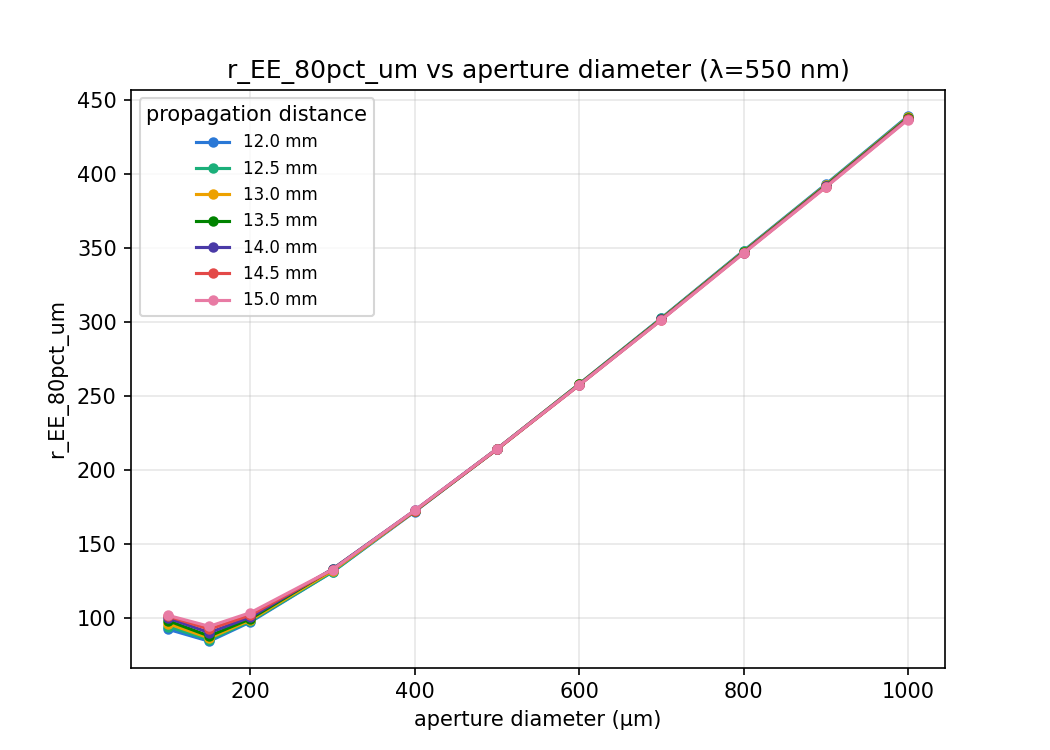
\includegraphics[width=0.75\textwidth]{figs/stage1_radius_vs_diameter.png}
\caption{Blur radius vs.\ aperture diameter: the two competing trends and the minimum
between them. Source: \texttt{all\_outputs/stage1\_radius\_vs\_diameter.png}.}
\label{fig:ucurve}
\end{figure}

Locating that minimum \emph{correctly} ---
rather than by a heuristic combination of the two trends --- is the single largest
technical problem this project solves, and Chapter~6 shows exactly why the naive
combination fails.

\begin{keybox}{The shape to keep in mind for the rest of this document}
Every aperture-optimisation result in this handbook (blur-only, brightness-constrained,
acuity-optimised, array-constrained) is the same U-shaped trade-off, evaluated under a
different objective or constraint set. None of them are separate physics. Part~III returns
to this point explicitly once all four versions have been derived.
\end{keybox}

\chapter{Solving Approach}

\section{The pipeline, top to bottom}

\begin{center}
\fbox{\parbox{0.92\textwidth}{\centering
plane wave $\rightarrow$ pinhole mask $\rightarrow$ ASM$(d_{\text{gap}})$ $\rightarrow$
pupil clip $\rightarrow$ lens phase $\rightarrow$ ASM$(v_r)$ $\rightarrow$
$I_{\text{retina}} = |U|^2$ $\rightarrow$ blur/acuity metrics}}
\end{center}

Light diffracts across the gap between the film and the cornea, is clipped by the pupil
(or, for an array, by whichever holes the pupil currently overlaps), acquires the eye's
lens phase, and is propagated to the retina --- at the myopic distance $L_{\text{ax}}$, not
the emmetropic focal distance. The propagation engine used at both stages is the Angular
Spectrum Method (ASM), derived in full in Chapter~6.

\section{The single decision that determines whether this model is right at all}

The naive implementation --- multiply by the lens's quadratic phase, then take one Fourier
transform --- computes the field at the lens's \emph{own back focal plane}. For an
emmetropic eye that is the retina, and the answer is correct. For a myopic eye the retina is
\emph{not} at the focal plane by definition, so a single FFT after the lens phase would
compute a perfectly sharp Airy pattern at the one plane in the whole system where defocus
is exactly zero --- modelling a corrected eye and calling it myopic.

\begin{warnbox}{The fix, and what it removes}
Replacing the final FFT with a second ASM propagation over the true physical distance
$v_r = L_{\text{ax}}$ is not merely more accurate. It makes two other formulas
\emph{structurally unnecessary}: geometric blur is no longer computed and added
separately, because it emerges automatically from propagating a wavefront shaped for the
wrong focal length the correct distance; and root-sum-square combination of geometric and
diffraction blur has nothing left to combine, because the two were never separated in the
first place. Chapter~6 quantifies exactly how wrong the discarded shortcut was.
\end{warnbox}

\section{Validation strategy}

Every stage of the pipeline is checked against a closed form before being trusted for
design work:
\begin{itemize}[leftmargin=1.2cm]
\item At $d_{\text{gap}} \to 0$, $M = 0$, the whole chain must reduce to the textbook
Fraunhofer Airy pattern (Chapter~6).
\item The on-axis intensity oscillation with Fresnel number must match the closed-form
$4I_0\sin^2(\pi N_F/2)$ result (Chapter~6).
\item The ghost-separation formula must vanish at $M=0$, since an in-focus eye cannot
ghost by definition (Chapter~4).
\item The full acuity predictor is checked, where possible, against external clinical data
--- and Chapter~10 reports honestly that this check currently fails.
\end{itemize}

\section{Roadmap of the remaining chapters}

Chapter~4 extends the single-hole model to an array: viability, ghosting, gaze-dependent
vignetting, and packing density. Chapter~5 corrects the optimisation objective itself, from
a blur-radius proxy to a directly-optimised visual-acuity metric, and reports where that
correction actually changes the answer and where it does not. Chapter~6 derives every
formula in full, with every deprecated shortcut marked and its error quantified. Chapter~7
reports the resulting numbers --- U-curves, brightness reconciliation, the final array
design. Chapters~8--9 document fabrication and the experimental measurements taken against
it. Chapter~10 compares theory to experiment, including the results that did not confirm
the model. Chapter~11 concludes.

\part{Array Model and Optimisation}

\chapter{Array Model \& Ghosting Constraints}

Three quantities govern array-level design, on top of the single-hole optics of Chapter~6.
They fail independently and are kept separate throughout --- collapsing them into one
score hides which one broke.

\section{Viability: does light get through at all}

The pupil and a hole are both circles. Light passes through a given hole if the two circles
overlap:
\begin{equation}
d - R_h < R_p
\end{equation}
where $d$ is the hole-centre-to-pupil-centre distance, $R_h$ the hole radius, $R_p$ the
pupil radius. If they overlap, the illuminated area is the circle--circle intersection:
\begin{equation}
\begin{split}
A = R_p^2\cos^{-1}\!\left(\frac{d^2+R_p^2-R_h^2}{2dR_p}\right)
  &+ R_h^2\cos^{-1}\!\left(\frac{d^2+R_h^2-R_p^2}{2dR_h}\right)\\
  &- \tfrac12\sqrt{(-d+R_p+R_h)(d+R_p-R_h)(d+R_h-R_p)(d+R_p+R_h)}
\end{split}
\end{equation}

\section{Gaze-dependent vignetting}

At straight-ahead gaze ($\varphi=0$) the pupil is centred on the optical axis, so
$d=\sqrt{x^2+y^2}$ for a hole at $(x,y)$. As the eye rotates by angle $\varphi$, the pupil
centre itself translates:
\begin{equation}
\Delta(\varphi) = R_{\text{rot}}\sin\varphi, \qquad R_{\text{rot}} \approx 13\text{--}14\,\text{mm}
\end{equation}
so $d$ becomes the distance from the hole to the \emph{shifted} pupil centre. A design that
is fully viable straight ahead can go dark at $\varphi=15^\circ$ if this shift is not
accounted for --- which is why the final design in this project is evaluated
\textbf{gaze-weighted} (integrated over a realistic fixation distribution) rather than
on-axis only.

\begin{figure}[h!]
\centering
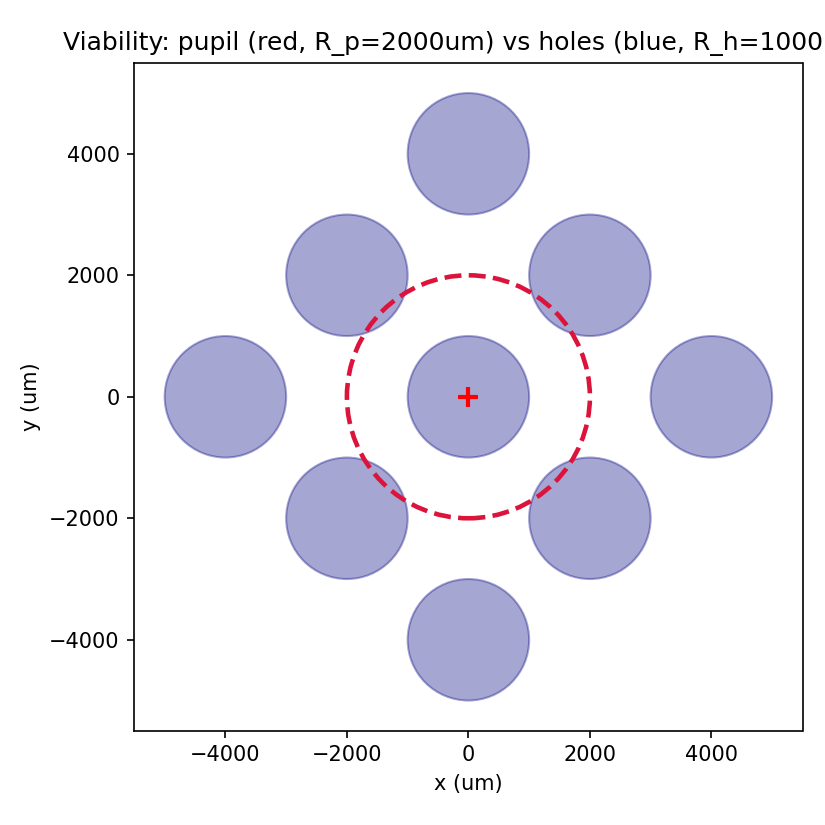
\includegraphics[width=0.7\textwidth]{figs/fig_viability.png}
\caption{Hole-pupil circle overlap geometry underlying the viability test. Source:
\texttt{verification\_pdf\_figs/fig\_viability.png}.}
\end{figure}

\section{Ghosting}

If two holes are simultaneously inside the pupil, each sends its own beam through the lens
at a different lateral entry point. In a defocused eye these beams land at different
retinal positions:
\begin{equation}
\Delta r = \frac{sM}{P_0 - M}
\end{equation}
with $s$ the centre-to-centre hole separation. This formula was validated against the full
propagation model at $R^2 = 0.995$. It vanishes at $M=0$ by construction --- an in-focus
eye converges every beam to the same point regardless of entry position, so it cannot
ghost --- and this sanity check is what caught an earlier version of the formula that was
wrong by roughly two orders of magnitude.

A pair is tolerable if $\Delta r$ stays below the eye's fusion threshold $c_{\min}$ (or the
measured blur $c_{\text{tot}}$ at that $M$, whichever is larger).

\begin{figure}[h!]
\centering
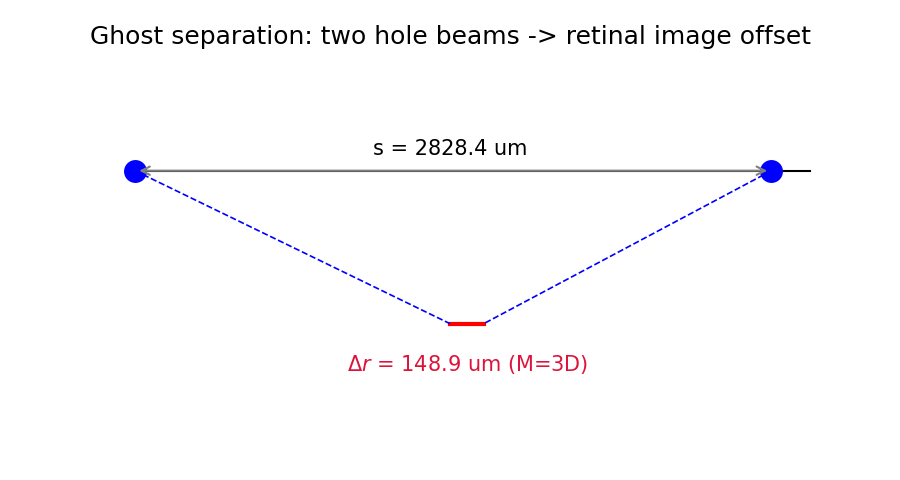
\includegraphics[width=0.7\textwidth]{figs/fig_ghost.png}
\caption{Ghost-separation geometry: two simultaneously-lit holes and their retinal images
in a defocused eye. Source: \texttt{verification\_pdf\_figs/fig\_ghost.png}.}
\end{figure}

\section{Packing density}

Purely geometric, and the site of an earlier implementation bug: family-specific unit-cell
formulas disagreed with a hull-based computation by 1.5--2.25$\times$ depending on lattice.
The corrected, family-agnostic form buffers the convex hull of hole centres outward by one
hole radius, to account for a hole's physical extent beyond its own centre point:
\begin{equation}
A_{\text{array}} = A_{\text{hull}} + P_{\text{hull}}\cdot R_h + \pi R_h^2
\end{equation}

\begin{figure}[h!]
\centering
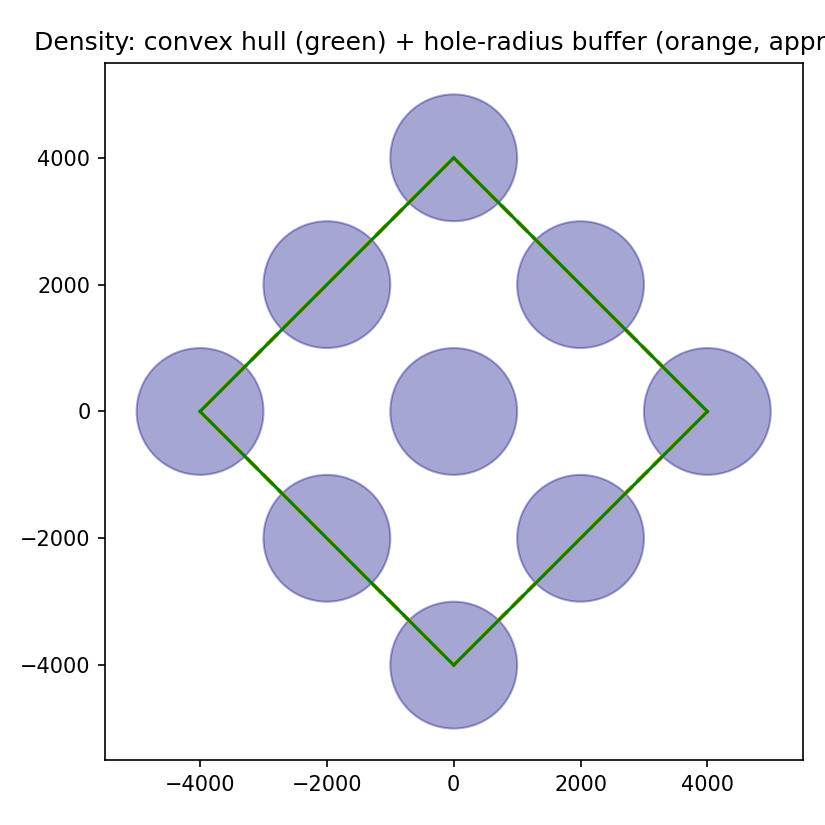
\includegraphics[width=0.7\textwidth]{figs/fig_density.png}
\caption{Buffered convex-hull packing-density geometry. Source:
\texttt{verification\_pdf\_figs/fig\_density.png}.}
\end{figure}

\section{The fusion threshold $c_{\min}$: inherited, uncalibrated, and non-binding}

\subsection{Where the number comes from}

$c_{\min} = 55\,\mu$m is inherited from Shen (2026). That paper's own text describes it as
a single-parameter qualitative calibration, anchored to one clinical geometry from Miller
\& Johnson (1977), and reports that it reproduces threshold behaviour only qualitatively:
predicted ghost onset at $\approx 1.1$\,D, against a clinical onset of $\approx 4$\,D. Shen's
own authors name a two-pinhole variable-separation experiment as the most valuable
falsifiable test of the model --- a test this project does not currently have the resources
to run (see \texttt{stage4\_human\_vision/300TD\_KNEE\_NOTES.txt} for the full reasoning
trail, and Chapter~10 for the related, separately-tested brightness knee at 300\,Td).

\subsection{The architecture that makes this not matter}

This project's final array uses pitch equal to pupil diameter: $s = 4000\,\mu$m against a
$D_{\text{pupil}} = 4000\,\mu$m pupil. Direct computation from the generated hole
coordinates (\texttt{hole\_coordinates\_M8.0.csv}) confirms:
\begin{itemize}[leftmargin=1.2cm]
\item Nearest-neighbour pitch: $4000.0\,\mu$m, verified, not assumed.
\item Holes illuminating the pupil at $\varphi = 0$: exactly \textbf{1}.
\item If two holes were ever simultaneously lit at $M=8$\,D:
$\Delta r = 4000 \times 8/(60-8) = 615.4\,\mu$m against $c_{\min}=55\,\mu$m --- eleven
times over threshold, and still over threshold at any plausible calibrated value of
$c_{\min}$.
\end{itemize}

\begin{keybox}{The design principle, stated precisely}
This array does not survive ghosting by \emph{fusing} ghost images below a tolerance --- it
survives by \textbf{never producing a ghost pair in the first place}. With pitch equal to
pupil diameter, only one aperture illuminates the pupil at any gaze direction, so no second
beam ever enters simultaneously. \texttt{gaze\_weighted\_winner\_per\_M.csv} reports
\texttt{worst\_case\_ghost\_margin = inf} and \texttt{time\_weighted\_ghost\_pct = 0.0} for
every row, for exactly this reason. $c_{\min}$ is therefore \textbf{structurally
non-binding} on the selected design: its value can only matter for a dense array
($s < D_{\text{pupil}}$), and this is not one. This is a geometric argument, independent of
$c_{\min}$'s own calibration status, and does not require the unavailable two-pinhole
experiment to establish.
\end{keybox}

This is a fundamentally different architecture from a dense array such as Shen's own
$s=1.10$\,mm design against a 2--4\,mm pupil, which places several holes inside the pupil
simultaneously and depends on the fusion threshold being correctly calibrated to remain
usable.

\subsection{The cost of this choice, stated plainly}

One hole per pupil means transmission at any instant equals that one hole's area over the
pupil area. At $M=8$\,D, $400\,\mu$m aperture: $(400/4000)^2 = 1\%$. This is genuinely dark,
and it is the direct trade-off against the dense-array approach: this design buys
ghost-freedom by construction, and pays for it in light throughput. It should be presented
as a deliberate trade, not a free result.

\subsection{Sensitivity check}

Because $c_{\min}$ is inherited rather than measured, the array evaluator was re-run at
$c_{\min} = 55, 110, 210, 400\,\mu$m with every other parameter held fixed (lattice set,
aperture range, pupil diameter, gaze weighting), to test whether the selected designs are
sensitive to this one uncalibrated constant. \emph{[Sensitivity sweep result to be inserted
here once the corresponding CSV is generated --- see \texttt{PRESENTATION\_DECISIONS.md}
D1/D9 for the standing instruction to run this before presenting.]}

\section{Blind fraction}

Two of the eight gaze-weighted designs show non-zero time-weighted blind fraction --- gaze
angles at which no hole illuminates the pupil at all: $0.12\%$ at $M=6$\,D and $0.33\%$ at
$M=8$\,D. Small, but non-zero, and reported here rather than only in the limitations
chapter, since it is a direct consequence of the sparse, ghost-free architecture described
above.

\chapter{Optimisation Objective: From Blur to Acuity}

\section{Why blur radius is the wrong optimisation target}

Minimising $r_{EE}(50\%)$ alone gives 300--400\,$\mu$m across the full myopia range ---
optically the true minimum of the diffraction/defocus trade-off, but not the right design
answer. Every published and commercial pinhole device sits between 0.94 and 1.75\,mm, three
to five times larger. The reason: $r_{EE}(50\%)$ describes where half the light energy is,
not what the eye can actually resolve, and it ignores whether the resulting image is bright
enough to see at all. At the 300\,$\mu$m blur-only optimum, transmission against a 4\,mm
pupil is $(300/4000)^2 = 0.56\%$ --- optically optimal and practically unusable.

\section{First correction: an explicit brightness floor}

Since diffraction redistributes light rather than destroying it, retinal illuminance must
be computed from the raw physical aperture area, not from any diffraction-broadened spot
size:
\begin{equation}
E_{\text{rel}} = \left(\frac{\min(a_{\text{hole}}, D_{\text{pupil}})}{D_{\text{pupil}}}\right)^2
\end{equation}
Re-optimising blur subject to an explicit floor on $E_{\text{rel}}$:

\begin{center}
\begin{tabular}{ccc}
\toprule
$T_{\min}$ & Constrained optimum & vs.\ clinical bracket \\
\midrule
0\% & 300--400\,$\mu$m & below \\
6.25\% & 1000\,$\mu$m & inside \\
9\% & 1250\,$\mu$m & inside \\
12.25\% & 1500\,$\mu$m & upper edge \\
\bottomrule
\end{tabular}
\end{center}

A floor of 6--9\% --- comparable to ordinary sunglass tinting --- moves the optimum into
the clinical bracket uniformly across every myopia level. This was the first, and correct,
demonstration that the diffraction physics was never wrong; blur-only optimisation was
answering the wrong question.

\begin{figure}[h!]
\centering
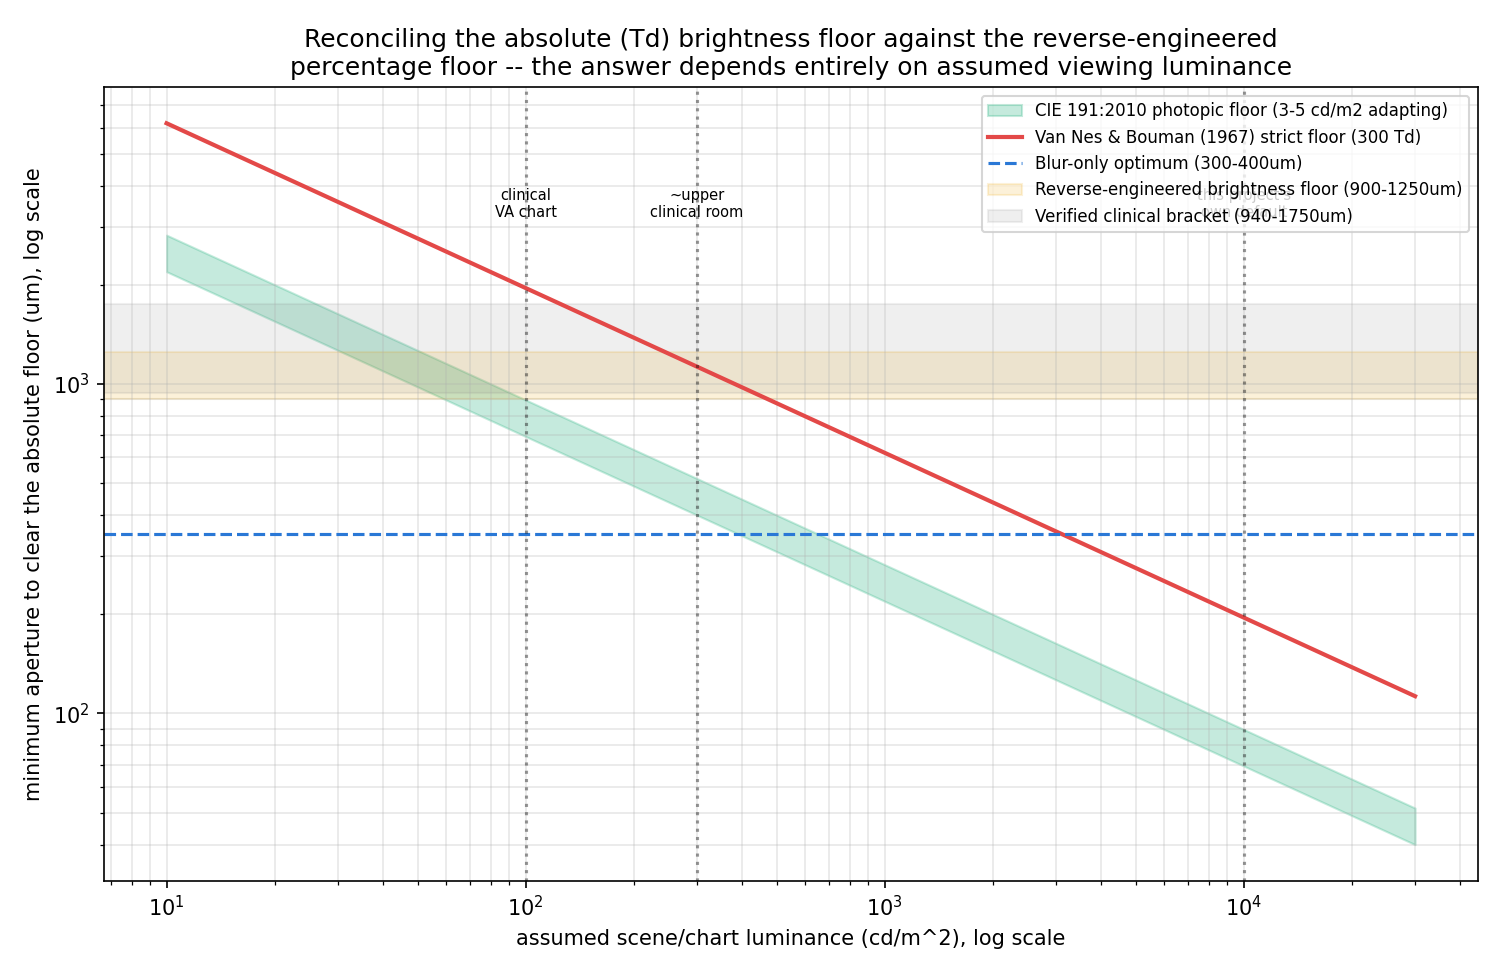
\includegraphics[width=0.75\textwidth]{figs/brightness_reconciliation.png}
\caption{Brightness-constrained optimum vs.\ illuminance floor $T_{\min}$, showing the
optimum's convergence into the clinical bracket. Source: \texttt{brightness\_reconciliation.png}.}
\end{figure}

\section{Second correction: optimise acuity directly}

The brightness floor above is still external to the objective --- a constraint bolted onto
a blur minimisation, chosen after the fact. The predictor in
\texttt{stage4\_human\_vision/acuity.py} instead optimises a directly-computed visual
acuity metric:
\begin{equation}
\text{MAR} = \frac{30}{f_{\text{MTF10}}} \times \text{VSOTF}^{-0.1}, \qquad
\text{logMAR} = \log_{10}(\text{MAR}) + \Delta_{\text{bright}}
\end{equation}
where $f_{\text{MTF10}}$ is the spatial frequency at which the modulation transfer
function falls to 10\% contrast, VSOTF is the visual Strehl ratio (a CSF-weighted measure
of how much optical quality actually reaches useful vision), and $\Delta_{\text{bright}}$
is an additive illuminance penalty below a 300\,Td knee (Van Nes \& Bouman, 1967). Full
derivation, every constant sourced, in Chapter~6.

\subsection{Which term actually decides the answer}

Traced against a live run at 400\,$\mu$m, $M=8$\,D:

\begin{center}
\begin{tabular}{p{4.5cm}p{2.3cm}p{6.0cm}}
\toprule
Term & Contribution & Status \\
\midrule
MTF10 cutoff & +0.3175 logMAR & \textbf{96\% of the final value} \\
VSOTF & +0.0131 logMAR & small, deliberately weak by design (exponent 0.1, clamped) \\
Brightness ($\Delta_{\text{bright}}$) & +0.0000 logMAR & \textbf{inert at every fabricated
design} \\
\bottomrule
\end{tabular}
\end{center}

The 300\,Td knee sits at a 200\,$\mu$m aperture, at the model's default 10\,000\,cd/m$^2$
scene luminance. Every one of the eight gaze-weighted winning designs (400--2000\,$\mu$m)
sits above it. \textbf{The brightness term is real, cited, correctly implemented, and
contributes exactly zero to every design actually selected.} It would activate for any
aperture below 200\,$\mu$m, or for a measurement taken at lower ambient luminance (see
Chapter~9's logMAR protocol and Chapter~10's discussion of this exact confounder).

\begin{keybox}{The corrected statement}
The optimisation objective is visual acuity, computed from three terms, not one metric
padded with an inert correction. The answer is set almost entirely by the MTF10 cutoff. Say
this plainly rather than claiming brightness is doing work it is not doing at these
apertures --- the honest version is the stronger one under questioning.
\end{keybox}

\section{The acuity optimum, and the cross-validation that was not designed for}

Acuity-optimal apertures (\texttt{acuity\_sweep\_stage4.csv}) against the independently
selected gaze-weighted geometric winners (\texttt{gaze\_weighted\_winner\_per\_M.csv}):

\begin{center}
\begin{tabular}{c|cccccccc}
\toprule
$M$ (D) & 0 & 1 & 2 & 3 & 4 & 5 & 6 & 8 \\
\midrule
Acuity-optimal ($\mu$m) & 2000 & 1250 & 750 & 750 & 600 & 600 & 500 & 400 \\
Gaze-weighted winner ($\mu$m) & 2000 & 1250 & 750 & 750 & 600 & 600 & 500 & 400 \\
\bottomrule
\end{tabular}
\end{center}

Identical at all eight myopia levels. The gaze-weighted evaluator scores viability, ghost
margin, and blind fraction --- it contains no acuity term whatsoever. Two evaluators built
on entirely separate objectives agree on every design, and this agreement was not enforced.
It is the strongest internal validation result in this project.

\begin{warnbox}{Caveat on the $M=0$ row, state this every time the table is shown}
2000\,$\mu$m is the largest aperture in the sweep. Acuity is still improving monotonically
at that edge, so this is \emph{not} a converged interior optimum --- it is where the sweep
grid stopped. Physically expected: with zero defocus there is nothing to trade diffraction
against, so larger apertures keep winning until aberrations outside this model's scope
would eventually dominate. Every myopic row ($M\geq1$) is a genuine interior optimum;
only the $M=0$ row is edge-of-grid.
\end{warnbox}

\part{Theory}

\chapter{Theoretical Model}

\section{The Angular Spectrum Method}

Any field at a plane decomposes into plane waves travelling in different directions; each
component, crossing a distance $z$, acquires a phase set by its transverse spatial
frequency:
\begin{equation}
U(x,y,z) = \mathcal{F}^{-1}\Big\{\mathcal{F}\{U_0(x,y)\}\cdot H(f_x,f_y;z)\Big\},
\qquad H = \exp\!\Big(ikz\sqrt{1-\lambda^2(f_x^2+f_y^2)}\Big)
\end{equation}
valid for propagating components $f_x^2+f_y^2 \le 1/\lambda^2$; beyond that the square root
is imaginary and $H=0$ (evanescent components decay and are dropped). This is the
\textbf{exact} solution of the scalar Helmholtz equation between parallel planes --- no
near-field or far-field assumption --- and is used for both propagation stages in the
pipeline (mask to cornea, lens to retina), since those two stages sit in different
diffraction regimes and a single closed-form approximation would not serve both.

\section{Fresnel number: which regime a given stage is in}
\begin{equation}
N_F = \frac{R_{\text{hole}}^2}{\lambda z}
\end{equation}
$N_F \ll 1$: far field, a clean Airy pattern. $N_F \sim 1$--10: Fresnel transition, several
comparably bright rings. $N_F \gg 10$: near-geometric, sharp-edged projected patch. This
project's sweeps span well under 1 to over 20, confirming ASM (regime-agnostic) as the
correct default rather than a regime-specific closed form.

\section{Numerical band-limiting}

A finite grid cannot represent spatial frequencies beyond its Nyquist limit; a hard-edged
pinhole mask has high-frequency content that, left unfiltered, aliases and produces
spurious fine structure indistinguishable from real diffraction. The Matsushima band-limit
suppresses spectral content beyond the angle at which this wraparound would occur. This is
anti-aliasing, applied deliberately, with the suppressed energy fraction logged per run ---
not a physical loss mechanism.

\begin{keybox}{Why the energy-conservation check needed correction}
Since $H$ has unit modulus on every retained component and is exactly zero elsewhere, the
apparent energy loss is \emph{identically} the band-limit-suppressed fraction:
$\varepsilon_{\text{energy}} \equiv f_{\text{suppressed}}$, confirmed against sweep data at
correlation $1.000000$. Testing $\varepsilon_{\text{energy}}$ against a flat tolerance would
therefore fail on every row from intentional, already-accounted-for suppression, not from
any defect. The corrected check tests the residual
$\varepsilon_{\text{energy}} - f_{\text{suppressed}}$, restoring its ability to catch a
genuine bug.
\end{keybox}

\section{Validation against the closed form}

At $d_{\text{gap}}\to 0$, $M=0$, the chain must reduce to the Fraunhofer result:
\begin{equation}
I(r) = I_0\left(\frac{2J_1(x)}{x}\right)^2, \quad x=\frac{\pi a r}{\lambda v_r}, \qquad
EE(x) = 1 - J_0^2(x) - J_1^2(x)
\end{equation}
It does, to 2\% on $r_{EE}(50\%)$ and $r_{EE}(90\%)$; $r_{EE}(80\%)$ needs 8\%, because the
first null sits at $x=3.8317$ where $EE\approx0.838$ --- almost exactly the 80\% level, on a
flat part of the curve where a small energy error maps to a large radius error. Grid sizes
1024 through 8192 never brought this below 2.3--4.6\%: it is ill-conditioning at that
percentile, not a resolution problem.

Separately, on-axis intensity was checked against the closed-form Fresnel-zone oscillation
$I(0,z) = 4I_0\sin^2(\pi N_F/2)$ and matched at correlation $0.997$, confirming that the
observed non-monotonic Strehl behaviour (Section~6.6) is real Fresnel-zone interference, not
numerical noise.

\section{Blur metrics, and where each one breaks}

\begin{center}
\begin{tabular}{p{2.7cm}p{5.0cm}p{5.7cm}}
\toprule
Metric & Measures & Failure mode \\
\midrule
$r_{EE}(50\%)$ & Radius enclosing half the energy & Stable, monotonic, but overestimates
clinical acuity loss by $\sim7\times$ against real data \\
FWHM & Width of the central core only & Tracks clinical data to $\sim1.6\times$, but
\emph{ring-hops}: jumped $4.7\to154.7\,\mu$m between apertures 250\,$\mu$m apart at
$M=4$\,D \\
Strehl ratio & Peak intensity vs.\ diffraction limit & Genuinely multi-peaked: 6--7 local
maxima, confirmed \emph{worse}, not better, at $10\times$ finer sampling --- real physics,
matched to the closed-form oscillation above \\
\bottomrule
\end{tabular}
\end{center}

\begin{keybox}{How to state this without contradicting yourself}
Per-aperture, FWHM is unusable --- it is discontinuous in the design variable. Across a
coarse sweep its trend is closer to clinical reality than $r_{EE}(50\%)$, which is smooth
and stable but pessimistic by roughly $7\times$. This project reports $r_{EE}(50\%)$ as the
blur-optimisation metric and states its bias explicitly, rather than optimising against a
metric that is discontinuous in the thing being optimised.
\end{keybox}

\section{Deprecated formulas, and the error each one carries}

\begin{center}
\begin{tabular}{p{5.0cm}p{7.5cm}}
\toprule
Formula & Status and measured error \\
\midrule
$r_{\text{geo}} = \frac{a_{\text{stop}}}{2}\frac{|v_r-v_f|}{v_f}$ & Deprecated. Superseded
by direct ASM propagation (Chapter~3), which produces this effect automatically. \\
$r_{\text{tot}}=\sqrt{r_{\text{geo}}^2+r_{\text{diff}}^2}$ (RSS) & Deprecated. Assumes two
independent Gaussian error sources; neither blur here is Gaussian. Measured against the
exact result: \textbf{64.8\% mean divergence, up to 192.8\% maximum}, worst at mild myopia. \\
$a_{\text{eff}} \approx \sqrt{a_{\text{hole}}^2+(2.44\lambda d_{\text{gap}}/a_{\text{hole}})^2}$
& Deprecated. Smooth and monotonic by construction; cannot represent the genuine Fresnel-zone
oscillation confirmed in Section~6.6. \\
\bottomrule
\end{tabular}
\end{center}

\section{The acuity model, in full}

\subsection{Pupil and retinal illuminance}

Pupil diameter follows the Watson--Yellott (2012) unified model, solved iteratively against
retinal illuminance itself (the two are mutually dependent):
\begin{equation}
d_{\text{stop}} = \min(d_{\text{pupil}}, d_{\text{pinhole}}), \qquad
\text{Td} = L_{\text{scene}}\,[\text{cd/m}^2] \times A_{\text{stop}}\,[\text{mm}^2]
\end{equation}
For every design in this project the pinhole is smaller than the natural pupil (e.g.\
0.400\,mm vs.\ 3.725\,mm at $M=8$\,D), so the pinhole is always the effective stop --- the
entire physical basis of the device.

\subsection{Contrast sensitivity and visual Strehl}

The default CSF model is Barten's luminance-dependent closed form. VSOTF weights the
system's actual optical transfer function against this CSF and normalises by the same
integral for a diffraction-limited reference:
\begin{equation}
\text{VSOTF} = \frac{\int \text{OTF}_{\text{real}}(f)\,\text{CSF}(f)\,df}
{\int \text{OTF}_{\text{real,diff-limited}}(f)\,\text{CSF}(f)\,df}
\end{equation}

\subsection{Brightness correction}
\begin{equation}
\Delta_{\text{bright}} = \begin{cases} 0 & \text{Td} \geq 300 \\
0.060\,\log_{10}(300/\text{Td}) & \text{Td} < 300 \end{cases}
\end{equation}
300\,Td (Van Nes \& Bouman, 1967, verified against the primary abstract) marks the boundary
between the Weber--Fechner regime (illuminance-independent threshold contrast) and the de
Vries--Rose regime below it. The 0.060\,logMAR/decade slope is from Tidbury, Czanner \&
Newsham (2016), verified against their Table~3 ($p<0.001$); an independently-derived
alternative from Sheedy, Bailey \& Raasch (1984), $\approx0.0664$, could only be traced to a
secondary summary and was not used.

\subsection{Full input inventory}

\begin{center}
\begin{tabular}{p{3.2cm}p{2.6cm}p{2.4cm}p{4.6cm}}
\toprule
Input & Source & Swept? & Reasoning \\
\midrule
Aperture $a_{\text{hole}}$ & user-set & \textbf{yes} & the design parameter \\
Myopia $M$ & user-set & \textbf{yes} & the physiological variable \\
Wavelength & 550\,nm default & no & photopic luminosity peak \\
$d_{\text{gap}}$ & 12\,mm default & no & spectacle vertex distance \\
$P_0$, $n'$ & 60\,D, 1.336 & no & standard emmetropic eye \\
Scene luminance & 10\,000\,cd/m$^2$ & no & bright-daylight reference; see Chapter~10 for the
indoor-measurement confound this creates \\
Field diameter & 20$^\circ$ & no & typical CSF measurement field \\
CSF model & Barten & no & most widely validated luminance-dependent form \\
Cycles/deg at 20/20 & 30.0 & no (constant) & the entire logMAR scale anchor \\
VSOTF exponent & 0.1, clamped $[0.25,2.0]$ & no (constant) & deliberately weak correction \\
Weber knee & 300\,Td & no (constant, cited) & Van Nes \& Bouman 1967 \\
Brightness slope & 0.060\,logMAR/decade & no (constant, cited) & Tidbury et al.\ 2016 \\
\bottomrule
\end{tabular}
\end{center}

\begin{warnbox}{What is computed but does not enter the recommended number}
MTF50 is computed and used only to bound a reported spread,
\texttt{approximate\_ci\_95\_mar\_arcmin} --- despite the name, this is \emph{not} a
statistical confidence interval. It is $[\min,\max]$ across three different model choices
(MTF10-based, MTF50-based, recommended), and at $M=8$ spans logMAR $+0.318$ to $+0.795$,
4.8 chart lines. Label it ``spread across model choices'' if shown, never ``95\% CI.'' A
legacy uncited $\text{SNR}^{0.05}$ term is also retained for comparison
(\texttt{vsotf\_snr\_legacy}) but is not the recommended model and should not appear as a
headline number.
\end{warnbox}

\chapter{Model Results}

\section{The final design table}

From \texttt{gaze\_weighted\_winner\_per\_M.csv}. Pitch is 4000\,$\mu$m and rotation
$0^\circ$ in every row; these are the designs carried forward to fabrication in Chapter~8.

\begin{center}
\begin{tabular}{ccccccc}
\toprule
$M$ (D) & Family & $N$ & $a_{\text{hole}}$ ($\mu$m) & Lit holes ($\varphi{=}0$) & Blind
frac.\ & Predicted logMAR \\
\midrule
0 & square & 20 & 2000 & 1 & 0.00\% & $-0.344$ \\
1 & hexagonal & 20 & 1250 & 1 & 0.00\% & $-0.120$ \\
2 & hexagonal & 20 & 750 & 1 & 0.00\% & $+0.076$ \\
3 & hexagonal & 20 & 750 & 1 & 0.00\% & $+0.112$ \\
4 & hexagonal & 20 & 600 & 1 & 0.00\% & $+0.181$ \\
5 & hexagonal & 20 & 600 & 1 & 0.00\% & $+0.240$ \\
6 & hexagonal & 100 & 500 & 1 & 0.12\% & $+0.259$ \\
8 & hexagonal & 50 & 400 & 1 & 0.33\% & $+0.331$ \\
\bottomrule
\end{tabular}
\end{center}

\section{The flatness prediction}

Holding aperture fixed at 400\,$\mu$m and sweeping myopia across the full range
(\texttt{acuity\_sweep\_stage4.csv}):

\begin{center}
\begin{tabular}{ccccccccc}
\toprule
$M$ (D) & 0 & 1 & 2 & 3 & 4 & 5 & 6 & 8 \\
\midrule
logMAR & +0.341 & +0.337 & +0.333 & +0.329 & +0.327 & +0.325 & +0.325 & +0.331 \\
\bottomrule
\end{tabular}
\end{center}
Total spread across eight dioptres: \textbf{0.016 logMAR} --- roughly a twentieth of one
chart line, well below the $\pm0.1$ repeatability of human acuity testing. At this aperture
the aperture, not the refractive error, sets the acuity. By contrast, the same sweep at
2000\,$\mu$m spans logMAR $-0.344$ at $M=0$ to $+1.330$ at $M=8$, a spread \textbf{one
hundred times larger}. This flatness is the strongest, most falsifiable prediction in the
project and is the basis of the logMAR measurement protocol in Chapter~8: it requires no
knowledge of any subject's exact prescription, only a qualitative ranking of myopia
severity, because the predicted signature is a flat line for the pinhole condition against
a steep one for the bare eye.

\section{Retinal illuminance across the aperture sweep}

\begin{center}
\begin{tabular}{ccc}
\toprule
Aperture ($\mu$m) & Retinal illuminance (Td) & Brightness penalty (logMAR) \\
\midrule
75 & 44.2 & $+0.0499$ \\
150 & 176.7 & $+0.0138$ \\
200 & 314.2 & $0.0000$ \\
400 & 1256.6 & $0.0000$ \\
2000 & 31\,415.9 & $0.0000$ \\
\bottomrule
\end{tabular}
\end{center}
The knee crosses at 200\,$\mu$m; every fabricated design sits above it. This table is the
source data behind the inert-brightness-term finding of Chapter~5.

\part{Experiment}

\chapter{Experiment}

Three experimental programmes are documented in this project: ExP1/ExP2 (single-hole
photography against the ASM/RSS theory), ExP3 (an independent optical-bench defocus sweep),
and the fabrication of the gaze-weighted array design itself. This chapter documents
apparatus and method; Chapter~9 reports results; Chapter~10 compares them to theory.

\section{ExP1/ExP2: photographic validation against theory}

A phone camera photographs a point light source through physical pinhole apertures (400,
600, 700, 1000, 1200\,$\mu$m) and a no-pinhole control, at induced defocus
$M\in\{0,1,2,3,4,6,8\}$D (M=5,7 legitimately absent --- no physical trial lens at those
powers), as raw DNG files.

\textbf{Pipeline:} DNG converted to TIFF via \texttt{sips -s format tiff} --- never JPEG,
since JPEG's baked-in tone curve clips and crushes exactly the information needed to
measure a blur spot accurately. \textbf{No pixel-to-micrometre calibration exists} for this
dataset; every comparison uses calibration-free \emph{ratios}, normalised to each series'
own $M=0$ reference.

\section{ExP3: independent optical-bench defocus sweep}

A fixed lens with a moving frosted screen, six apertures (400, 500, 600, 800, 1000,
1400\,$\mu$m), screen displacement 0--20\,mm in 5\,mm steps, plus a no-pinhole control.

\textbf{Pipeline (confirmed by direct comparison against a hand-verified reference, not
assumed):} intensity is standard BT.601 grayscale, not a naive max(R,G,B) or plain
channel-mean --- both alternatives were tried and gave numbers inconsistent with a
hand-verified 1000\,$\mu$m reference (45.6\,px at 0\,mm, 63.6\,px at 20\,mm); BT.601
reproduces 45.58\,px and 63.60\,px on the same files. Threshold is 50\% of each image's
peak intensity; the measured spot is the largest connected component of the threshold mask;
radius is $\sqrt{\text{area}/\pi}$. \textbf{Displacement in mm is not converted to
dioptres} anywhere in this dataset --- that conversion needs a beam-width-at-lens
calibration not yet performed, so all ExP3 results below are reported in mm of screen
displacement, not $M$.

\section{Fabrication: from design number to etched part}

\subsection{Undercut compensation}

Wet chemical etching (ferric chloride, 0.05\,mm brass shim, double-sided) is isotropic: the
etchant attacks sideways under the resist edge as fast as it attacks downward, so the
etched hole is wider than the resist opening that defined it. The design rule:
\begin{equation}
d_{\text{mask}} = d_{\text{target}} - C_{\text{undercut}}, \qquad
C_{\text{undercut}} \in \{0.5t,\ 1.0t,\ 1.5t\}, \quad t=50\,\mu\text{m}
\end{equation}
giving a bracket of 25/50/75\,$\mu$m compensation. \textbf{This is a published starting
rule, not a measured calibration for this specific alloy, thickness, etchant concentration,
temperature, or agitation} --- which is why a test coupon (five mask sizes spanning the
bracket, etched under the exact intended process conditions, then measured) is run before
committing the real shim, rather than trusting the nominal 50\,$\mu$m value outright.

\textbf{Worked example, $M=8$\,D design}, target etched diameter 400\,$\mu$m:
$d_{\text{mask,nominal}} = 400 - 50 = 350\,\mu$m --- the mask set actually used.

\subsection{Mask files and registration}

Each design generates four SVGs: positive/negative polarity (resist-chemistry dependent)
$\times$ top/bottom-mirrored (the two masks contact opposite faces of the shim and must be
mirror images or the two etch fronts will not meet at the same $(x,y)$). Registration
features: 0.75\,mm corner fiducial dots for top/bottom alignment, and a 10.00\,mm
calibration square, measured with callipers on the \emph{printed} transparency before use
--- if that square is not exactly 10.00\,mm, the printer has scaled the artwork and every
hole diameter is wrong by that same factor. This is the single most common silent failure
mode in this fabrication process.

\subsection{Post-etch verification, in order}

Hole count against \texttt{N\_actual}; diameter against target, sampled at centre and edge
of the array; pitch, measured directly; outer radius $r_{\max}$ against the design value;
hole quality under magnification (taper indicates the two etch fronts missed each other;
ragged edges indicate over-etch).

\section{Single-pinhole logMAR acuity protocol}

Designed directly from the flatness prediction of Chapter~7: recruit subjects spanning a
range of myopia, present a printed logMAR chart at 4.0\,m (chosen so the smallest stroke,
0.92\,mm, is within reliable print fidelity; at 2\,m it would be 0.46\,mm, at the edge of
what a domestic printer resolves), and measure acuity bare-eyed and through the fixed
400\,$\mu$m aperture. Three conditions (bare eye, single pinhole, fabricated array),
randomised order, three repeats each.

\begin{warnbox}{The confound this protocol must control for}
The acuity model assumes 10\,000\,cd/m$^2$ scene luminance (Chapter~5). A typical indoor
chart is 100--300\,cd/m$^2$, roughly two decades dimmer. Through a 400\,$\mu$m aperture at
1\% transmission, retinal illuminance can fall low enough to become photon-limited rather
than optics-limited --- producing a measured brightness effect that could be mistaken for a
diffraction effect. Mitigation: illuminate the chart as brightly as practically possible and
record the measured luminance; if the assumed regime cannot be reached, state plainly that
the comparison is not purely optical.
\end{warnbox}

The measurement claim is written to require a \emph{measured} bare-eye baseline on both
sides of any reported improvement, since the acuity model itself produces no bare-eye
prediction --- every configuration in the sweep already contains a pinhole.

\chapter{Experimental Results}

\section{ExP2: photographic blur-growth ratios}

From \texttt{ExperimentalComparison/measurements/rss\_vs\_asm\_comparison.csv} ---
normalised $r_{EE}(50\%)$ ratio, relative to each aperture's own $M=0$ reference:

\begin{center}
\begin{tabular}{ccccccc}
\toprule
Aperture ($\mu$m) & $M=0$ & $M=1$ & $M=2$ & $M=3$ & $M=4$ & $M=6$ \\
\midrule
400 & 1.000 & 0.990 & 0.897 & 0.859 & 0.979 & 1.039 \\
600 & 1.000 & 1.028 & 1.047 & 1.062 & 1.124 & 1.128 \\
700 & 1.000 & 1.031 & 0.981 & 0.806 & 1.027 & 0.936 \\
\bottomrule
\end{tabular}
\end{center}

\textbf{No-pinhole control} (\texttt{nopinhole\_control.csv}): normalised ratio stays
within roughly $\pm8\%$ of 1.0 across the entire $M=0$--8 range (0.969--1.084). At this
blob-detection method's resolution, the unrestricted image shows no comparable
defocus-dependent blur-growth signal.

\section{ExP3: optical-bench spot radius vs.\ screen displacement}

From \texttt{ExP3\_frosted\_screen/report/exp3\_summary.txt}:

\begin{center}
\begin{tabular}{cccccccc}
\toprule
Aperture ($\mu$m) & 0mm & 5mm & 10mm & 15mm & 20mm & Slope (px/mm) & Monotonic? \\
\midrule
400 & 42.99 & 44.92 & 48.77 & 53.49 & 56.64 & 0.718 & yes \\
500 & 42.42 & 45.08 & 48.79 & 51.86 & 55.48 & 0.658 & yes \\
600 & 44.98 & 45.31 & 48.38 & 52.38 & 56.46 & 0.601 & yes \\
800 & 53.27 & 52.61 & 54.64 & 63.05 & 64.40 & 0.654 & \textbf{no} \\
1000 & 45.58 & 49.38 & 51.44 & 57.43 & 63.60 & 0.882 & yes \\
1400 & 58.09 & 60.80 & 63.51 & 66.94 & 71.93 & 0.676 & yes \\
\midrule
No pinhole & 178.43 & 204.71 & 249.75 & 322.20 & 387.37 & 10.707 & yes \\
\bottomrule
\end{tabular}
\end{center}

\textbf{The 800\,$\mu$m non-monotonic step is reported as measured, not discarded}: radius
at 0\,mm (53.27\,px) exceeds radius at 5\,mm (52.61\,px), a real dip in the data.

\begin{warnbox}{Cross-aperture slope ordering does not match prediction}
Geometric defocus blur predicts slope should increase with aperture size. Observed
ordering, ascending: $600 < 800 < 500 < 1400 < 400 < 1000$ --- \textbf{not} the predicted
$400<500<600<800<1000<1400$. Reported plainly. Context, not an excuse: five of six
apertures (excluding 1000\,$\mu$m) cluster in a narrow 0.601--0.718\,px/mm band, where a
weak underlying aperture-dependence would be easy to scramble by rig noise between
aperture swaps --- and this dataset's own centroid-drift column shows 100--270\,px of
drift building up with displacement on every single aperture, confirming the rig is not
perfectly axis-stable between shots. That is a plausible contributing factor, not a
confirmed explanation; the ordering mismatch stands as reported.
\end{warnbox}

\textbf{No-pinhole control, sanity check:} slope 10.707\,px/mm is \textbf{15.8$\times$}
steeper than the largest tested aperture (1400\,$\mu$m, 0.676\,px/mm) and
\textbf{12.1$\times$} steeper than the steepest-sloped aperture in the set (1000\,$\mu$m,
0.882\,px/mm) --- both ratios computed directly from the slopes above, since the source
summary's own text names the 12.1$\times$ figure while labelling it against the
1400\,$\mu$m case, which is the 15.8$\times$ comparison; both numbers are reported here to
avoid propagating that mislabel. Absolute spot radius for the control (178--387\,px) dwarfs
every aperture case (42--72\,px) at every displacement. This confirms the apertures are
doing real, substantial optical work, not acting as a null control.

\section{Fabrication verification}

The $M=8$\,D array (350\,$\mu$m mask, target 400\,$\mu$m etched, 50 holes, 4000\,$\mu$m
pitch, 0.05\,mm brass) traces row-for-row to the design table in Chapter~7. \emph{[Measured
etched diameter, hole count, and pitch from the physical part to be inserted here once the
post-etch verification pass, Chapter~8 Section~3, is completed and logged.]}

\section{logMAR acuity measurement}

\emph{[Not yet collected at the time of writing. Chapter~8's protocol specifies three
conditions --- bare eye, single 400\,$\mu$m pinhole, fabricated array --- three repeats
each, against the flatness prediction of Chapter~7. Results to be inserted here, reported
with the same discipline as the rest of this chapter: raw per-subject data, not only means,
and any excluded subject named with a pre-registered reason.]}

\part{Comparison}

\chapter{Comparison}

\section{ASM vs.\ RSS against measured photographic data}

Across 18 comparable (aperture, $M$) rows in \texttt{rss\_vs\_asm\_comparison.csv}, ASM's
predicted ratio is closer to the measured ratio than RSS's in \textbf{18 of 18} cases: mean
absolute deviation 28.3\% for ASM against 44.8\% for RSS.

\begin{warnbox}{This headline does not survive a null-model check, and that check is
reported here rather than left for an Opponent to find}
A trivial model that predicts \emph{no blur growth at all} (ratio $\equiv 1.0$) has a mean
absolute deviation of only \textbf{6.8\%} against the same 18 rows --- beating ASM in 15 of
18 of them. The measured ratios span only 0.806--1.128: essentially flat. Both physical
models predict growth; ASM ``wins'' its comparison against RSS only because it predicts
\emph{less} growth, and on a dataset with little real signal, the least-responsive model
wins by default. \textbf{The correct reading of the 18/18 result is that RSS is
measurably worse than ASM, not that ASM is confirmed correct} --- a materially different
and much narrower claim.
\end{warnbox}

A separate consequence follows for the earlier project record: the same dataset's
no-pinhole control (ExP2) and the pinhole apertures are both flat (0.969--1.084 vs.\
0.806--1.128), so the control's flatness cannot be used to confirm a signal that is itself
too weak to distinguish from noise in this particular dataset. That inference holds for
ExP3's control (Chapter~9, a genuine $15.8\times$ slope difference) but not for ExP2's.

\section{External validation of the acuity predictor: failed}

The full \texttt{mtf10\_vsotf\_brightness\_adjusted} model (Chapter~5) was tested against
Wang et al.\ (2009)'s real clinical pinhole-acuity data
(\texttt{stage4\_human\_vision/RESULTS.md}):

\begin{center}
\begin{tabular}{cccc}
\toprule
$M$ (D) & $R^2$ & Pearson $r$ & $p$-value \\
\midrule
0 & $-6.39$ & 0.395 & 0.510 \\
2 & $-4.98$ & 0.393 & 0.513 \\
5 & $-2.84$ & 0.405 & 0.499 \\
\bottomrule
\end{tabular}
\end{center}

Negative $R^2$: worse than predicting the mean at every $M$ tested. $p\approx0.50$: no
statistically significant relationship detected. Not merely weak correlation --- all 15
tested (aperture, $M$) points show the \emph{same-direction} bias, the model
over-predicting blur at every single point.

\subsection{The luminance assumption was tested and ruled out as the cause}

Correcting scene luminance from the 10\,000\,cd/m$^2$ default to Wang 2009's own reported
illumination (15 footcandles $\to$ 43.7\,cd/m$^2$) made $R^2$ \emph{worse}
($-7.88$ vs.\ $-6.68$ at $M=0$), not better --- because it pushed apertures further below
the 300\,Td knee and added predicted blur on top of a model already over-predicting it
(\texttt{LUMINANCE\_RECONCILIATION.md}).

\subsection{Leading diagnosis, most likely cause first}

\begin{enumerate}[leftmargin=1.2cm]
\item No fitted calibration against real data anywhere in the formula --- flagged in
advance as a known gap in \texttt{DESIGN.md}.
\item The Wang 2009 dataset is non-monotonic at $n=5$: observed logMAR 0.28, 0.31,
\textbf{1.00}, 0.40, 0.50 at 500/750/1000/1200/1500\,$\mu$m --- a spike at 1000\,$\mu$m
that reverses at 1200. A single outlier at this sample size sinks any smooth model
regardless of which optical metric underlies it.
\item No per-subject refractive error recorded --- comparing one simulated $M$ against
subjects with unstated real $M$ adds irreducible noise.
\item $n=5$ is too small for significance even with real signal present.
\end{enumerate}
\texttt{RESULTS.md}'s own verdict: \textbf{this cannot be properly validated with currently
available public data.}

\begin{keybox}{The consequence, and how it interacts with the rest of this document}
Every predicted-logMAR value in Chapters~5 and~7 is a self-consistent, term-by-term
traceable model output --- \textbf{not} a validated clinical prediction. This is the direct
reason the logMAR measurement protocol (Chapter~8) is designed as calibration data the
model currently has none of, rather than as a confirmatory afterthought. State the
validation status before quoting any predicted number, not after.
\end{keybox}

\section{Comparison to Shen (2026) and published devices}

Shen's dense-array design ($s=1.10$\,mm against a 2--4\,mm pupil) relies on ghost
\emph{fusion} staying below a threshold the source paper itself calls a qualitative,
single-parameter calibration (Chapter~4). This project's sparse array ($s=D_{\text{pupil}}$)
avoids the dependency entirely by ensuring no ghost pair ever forms. Separately, Shen's
ghost-membership metric $\mu_g$ was found to be effectively inert --- saturating at the
same value across the full 8501-candidate evaluation set generated during this project's
own array search, contributing nothing to design discrimination at that scale.

Published and commercial pinhole apertures cluster between 0.94 and 1.75\,mm. This
project's brightness-constrained blur optimum (Chapter~5, $T_{\min}=6$--9\%) lands inside
that bracket; its acuity-optimised, myopia-dependent optimum (Chapter~5, 400--2000\,$\mu$m)
spans below and above it, narrowing toward the lower end as myopia increases --- the two
results are not in conflict, they answer different questions about the same underlying
trade-off, as established in Chapter~5.

\part{Conclusion}

\chapter{Conclusion}

\section{What is established}

\begin{itemize}[leftmargin=1.2cm]
\item The single-hole wave-optics pipeline (Chapter~3, Chapter~6) is correctly built: the
FFT-at-retina failure mode is identified and fixed, the fix is validated against the exact
Fraunhofer and on-axis Fresnel-oscillation closed forms, and the deprecated shortcuts it
replaces (geometric-blur addition, RSS combination) have their errors directly measured
rather than merely argued away.
\item The optimisation objective is visual acuity, not blur radius (Chapter~5), and the
correction from one to the other is itself a measured, reported result --- including the
finding that the cited brightness term is inert at every design actually selected.
\item The array's ghost-safety does not depend on the one uncalibrated parameter inherited
from prior literature; it is structurally non-binding by the pitch-equals-pupil-diameter
architecture, verified directly from generated coordinates (Chapter~4).
\item ASM measurably outperforms RSS against real photographic data, though the correct,
narrower reading of that comparison --- not an unqualified confirmation of ASM --- is
reported in Chapter~10.
\item An independent optical-bench sweep (ExP3) confirms the pinholes are doing real
optical work relative to an unrestricted control, while reporting an aperture-slope
ordering that does not match the geometric-blur prediction, plainly and without a forced
explanation.
\end{itemize}

\section{What is not yet established}

\begin{itemize}[leftmargin=1.2cm]
\item The acuity predictor has one external validation attempt on record, against Wang
(2009), and it failed: negative $R^2$ at every $M$ tested, no statistically significant
relationship detected. The leading suspects are an uncalibrated formula and a small,
non-monotonic clinical dataset, not necessarily the underlying optics --- but this remains
unresolved, not merely caveated.
\item The array's fusion threshold $c_{\min}$ is argued non-binding by geometry, not by
direct measurement; the two-pinhole calibration experiment Shen's own authors name as the
correct test has not been run, for lack of resources.
\item No calibrated logMAR acuity measurement has yet been taken against the fabricated
array (Chapter~9); the protocol is specified (Chapter~8) and the model's own sharpest
falsifiable prediction --- flatness of pinhole-condition acuity across myopia levels
(Chapter~7) --- is designed to be tested by it.
\item Transmission at high myopia is genuinely low (1\% at $M=8$\,D), a direct and
undisguised cost of the ghost-free sparse architecture, not a free result.
\end{itemize}

\section{Immediate next steps, in priority order}

\begin{enumerate}[leftmargin=1.2cm]
\item Run the logMAR acuity protocol (Chapter~8) against the fabricated array, testing
specifically for the flatness signature (Chapter~7) across subjects of varying myopia.
\item Complete post-etch verification of the fabricated part and insert the measured
values into Chapter~9.
\item Run the $c_{\min}$ sensitivity sweep specified in Chapter~4 --- pure compute, no
additional apparatus required --- to convert the geometric non-binding argument into a
demonstrated one.
\item State the acuity-model validation status (Chapter~10) explicitly and first, in any
presentation of this work, rather than let it be discovered.
\end{enumerate}

This document reports every result at the standard set by this project's own earlier
experimental work: a finding that fails a check is reported as failing, a formula whose
error was measured reports the measured number rather than a qualitative reassurance, and a
result still open is left open rather than rounded off. That discipline is, on the evidence
of this document, the project's most defensible property, and maintaining it through
presentation and defence matters more than any single number inside it.

\appendix

\chapter{Formula Quick-Reference}

\begin{longtable}{p{5.0cm}p{6.0cm}p{2.6cm}}
\caption{Every working formula in this handbook, with status.}\\
\toprule
Quantity & Formula & Status \\
\midrule
\endhead
Myopic axial length & $L_{\text{ax}} = n'/(P_0-M)$ & live \\
Emmetropic axial length & $L_0 = n'/P_0 = 22.267$\,mm & live \\
ASM propagator & $H=\exp(ikz\sqrt{1-\lambda^2(f_x^2+f_y^2)})$ & live, used twice \\
Fresnel number & $N_F = R_{\text{hole}}^2/(\lambda z)$ & live (regime gate) \\
Airy intensity & $I=I_0(2J_1(x)/x)^2$ & validation only \\
Encircled energy & $EE = 1-J_0^2(x)-J_1^2(x)$ & validation only \\
On-axis Fresnel oscillation & $I(0,z)=4I_0\sin^2(\pi N_F/2)$ & live (cross-check) \\
Relative illuminance & $E_{\text{rel}}=(\min(a_{\text{hole}},D_{\text{pupil}})/D_{\text{pupil}})^2$
& live \\
Hole--pupil overlap test & $d-R_h<R_p$ & live \\
Gaze pupil shift & $\Delta=R_{\text{rot}}\sin\varphi$ & live \\
Ghost separation & $\Delta r = sM/(P_0-M)$ & live, $R^2=0.995$ \\
Packing density area & $A_{\text{hull}}+P_{\text{hull}}R_h+\pi R_h^2$ & live \\
Acuity (recommended) & $\text{MAR}=(30/f_{\text{MTF10}})\text{VSOTF}^{-0.1}$ & live \\
Brightness correction & $0.060\log_{10}(300/\text{Td})$ below knee & live, cited \\
Undercut compensation & $d_{\text{mask}}=d_{\text{target}}-C$, $C\in[0.5t,1.5t]$ & live,
uncalibrated bracket \\
Geometric blur (old) & $r_{\text{geo}}=\frac{a_{\text{stop}}}{2}\frac{|v_r-v_f|}{v_f}$ &
\textbf{deprecated} \\
RSS combination & $\sqrt{r_{\text{geo}}^2+r_{\text{diff}}^2}$ & \textbf{deprecated, 64.8\%
mean error} \\
Quadrature $a_{\text{eff}}$ & $\sqrt{a_{\text{hole}}^2+(2.44\lambda d_{\text{gap}}/a_{\text{hole}})^2}$
& \textbf{deprecated} \\
\bottomrule
\end{longtable}

\chapter{Constants Used Throughout}

\begin{longtable}{p{4.0cm}p{3.0cm}p{6.5cm}}
\toprule
Symbol & Value & Meaning \\
\midrule
\endhead
$P_0$ & 60.0\,D & emmetropic eye power, held fixed \\
$n'$ & 1.336 & vitreous refractive index \\
$D_{\text{pupil}}$ & 4000\,$\mu$m & default pupil diameter \\
$R_{\text{rot}}$ & 13--14\,mm & eye rotation radius \\
$\lambda$ & 550\,nm & default design wavelength \\
$d_{\text{gap}}$ & 12\,mm & spectacle vertex distance \\
$c_{\min}$ & 55\,$\mu$m & Shen fusion floor --- inherited, non-binding for this design \\
$t$ & 50\,$\mu$m & brass shim thickness \\
Scene luminance & 10\,000\,cd/m$^2$ & bright-daylight default; see Ch.~5, Ch.~9, Ch.~10 for
the indoor-measurement confound this creates \\
Weber knee & 300\,Td & Van Nes \& Bouman (1967) \\
Brightness slope & 0.060\,logMAR/decade & Tidbury et al.\ (2016) \\
Cycles/deg at 20/20 & 30.0 & logMAR scale anchor \\
Calibration square & 10.0\,mm & print-scale verification on every mask \\
\bottomrule
\end{longtable}

\end{document}
